\chapter{LwM2M}

Il est temps de voir une vrai plateforme IoT qui met en œuvre ce que nous venons d'apprendre sur CoAP et REST. Il faut installer deux programmes \Index{java}\footnote{Il s'agit d'une mise en œuvre assez ancienne, de nouvelles spécifications existent et sont quelque peu différentes, mais les concepts n'ont pas changés}~:

\begin{termc}[backgroundcolor=\color{verttelecom!30}, basicstyle=\ttfamily\tiny, escapechar=@]
wget https://ci.eclipse.org/leshan/job/leshan/lastSuccessfulBuild/artifact/leshan-client-demo.jar
\end{termc}

\noindent et

\begin{termc}[backgroundcolor=\color{verttelecom!30}, basicstyle=\ttfamily\tiny, escapechar=@]
wget https://ci.eclipse.org/leshan/job/leshan/lastSuccessfulBuild/artifact/leshan-server-demo.jar
\end{termc}

\section{Introduction}

\ac{LwM2M} est une architecture définie par l'\ac{OMA} à l'origine pour permettre aux opérateurs de gérer certaines ressources sur les téléphones mobiles. Mais cette architecture peut être étendu à d'autres environnement. 

         \vspace{1em}

Les spécifications sont accessibles sur le site de l'OMA\footnote{\url{https://omaspecworks.org/what-is-oma-specworks/iot/lightweight-m2m-lwm2m/}}. Nous allons utiliser une mise en œuvre en java appelé \index{Leshan}. Pas de panique nous n'allons pas programmer nous aurons juste besoin d'un navigateur Web et de \Index{Wireshark}.

         \vspace{1em}

\ac{LwM2M} comme son nom l'indique se veut léger, c'est-à-dire que les mises en œuvre ne doivent pas être trop complexes et que le trafic engendrer ne doit pas non plus être trop important. LwM2M est une plate-forme et elle va donc faire plus qu'un simple trafic REST. En particulier, l'un des rôles est de permettre aux objets de s'enregistrer et de décrire leurs caractéristiques. LmM2M va également structurer fortement les ressources en imposant des règles de nommages relativement contraintes et le format des ressources.

\section{Architecture}

Comme tout système qui se respecte, LwM2M fonctionne en mode client/serveur. Le serveur est la plate-forme de gestion des objets et les clients sont les objets connectés sur le réseau.

Dans un premier temps, lancez Wireshark sur l'interface \textit{\Index{loopback}} et filtrez le trafic en le limitant au port 5683 pour UDP (celui de CoAP) en tapant \texttt{udp.port==5683}. Comme le montre la figure~\vref{fig-lwm2m-wireshark}.

\begin{figure}[tbp]
\centerline{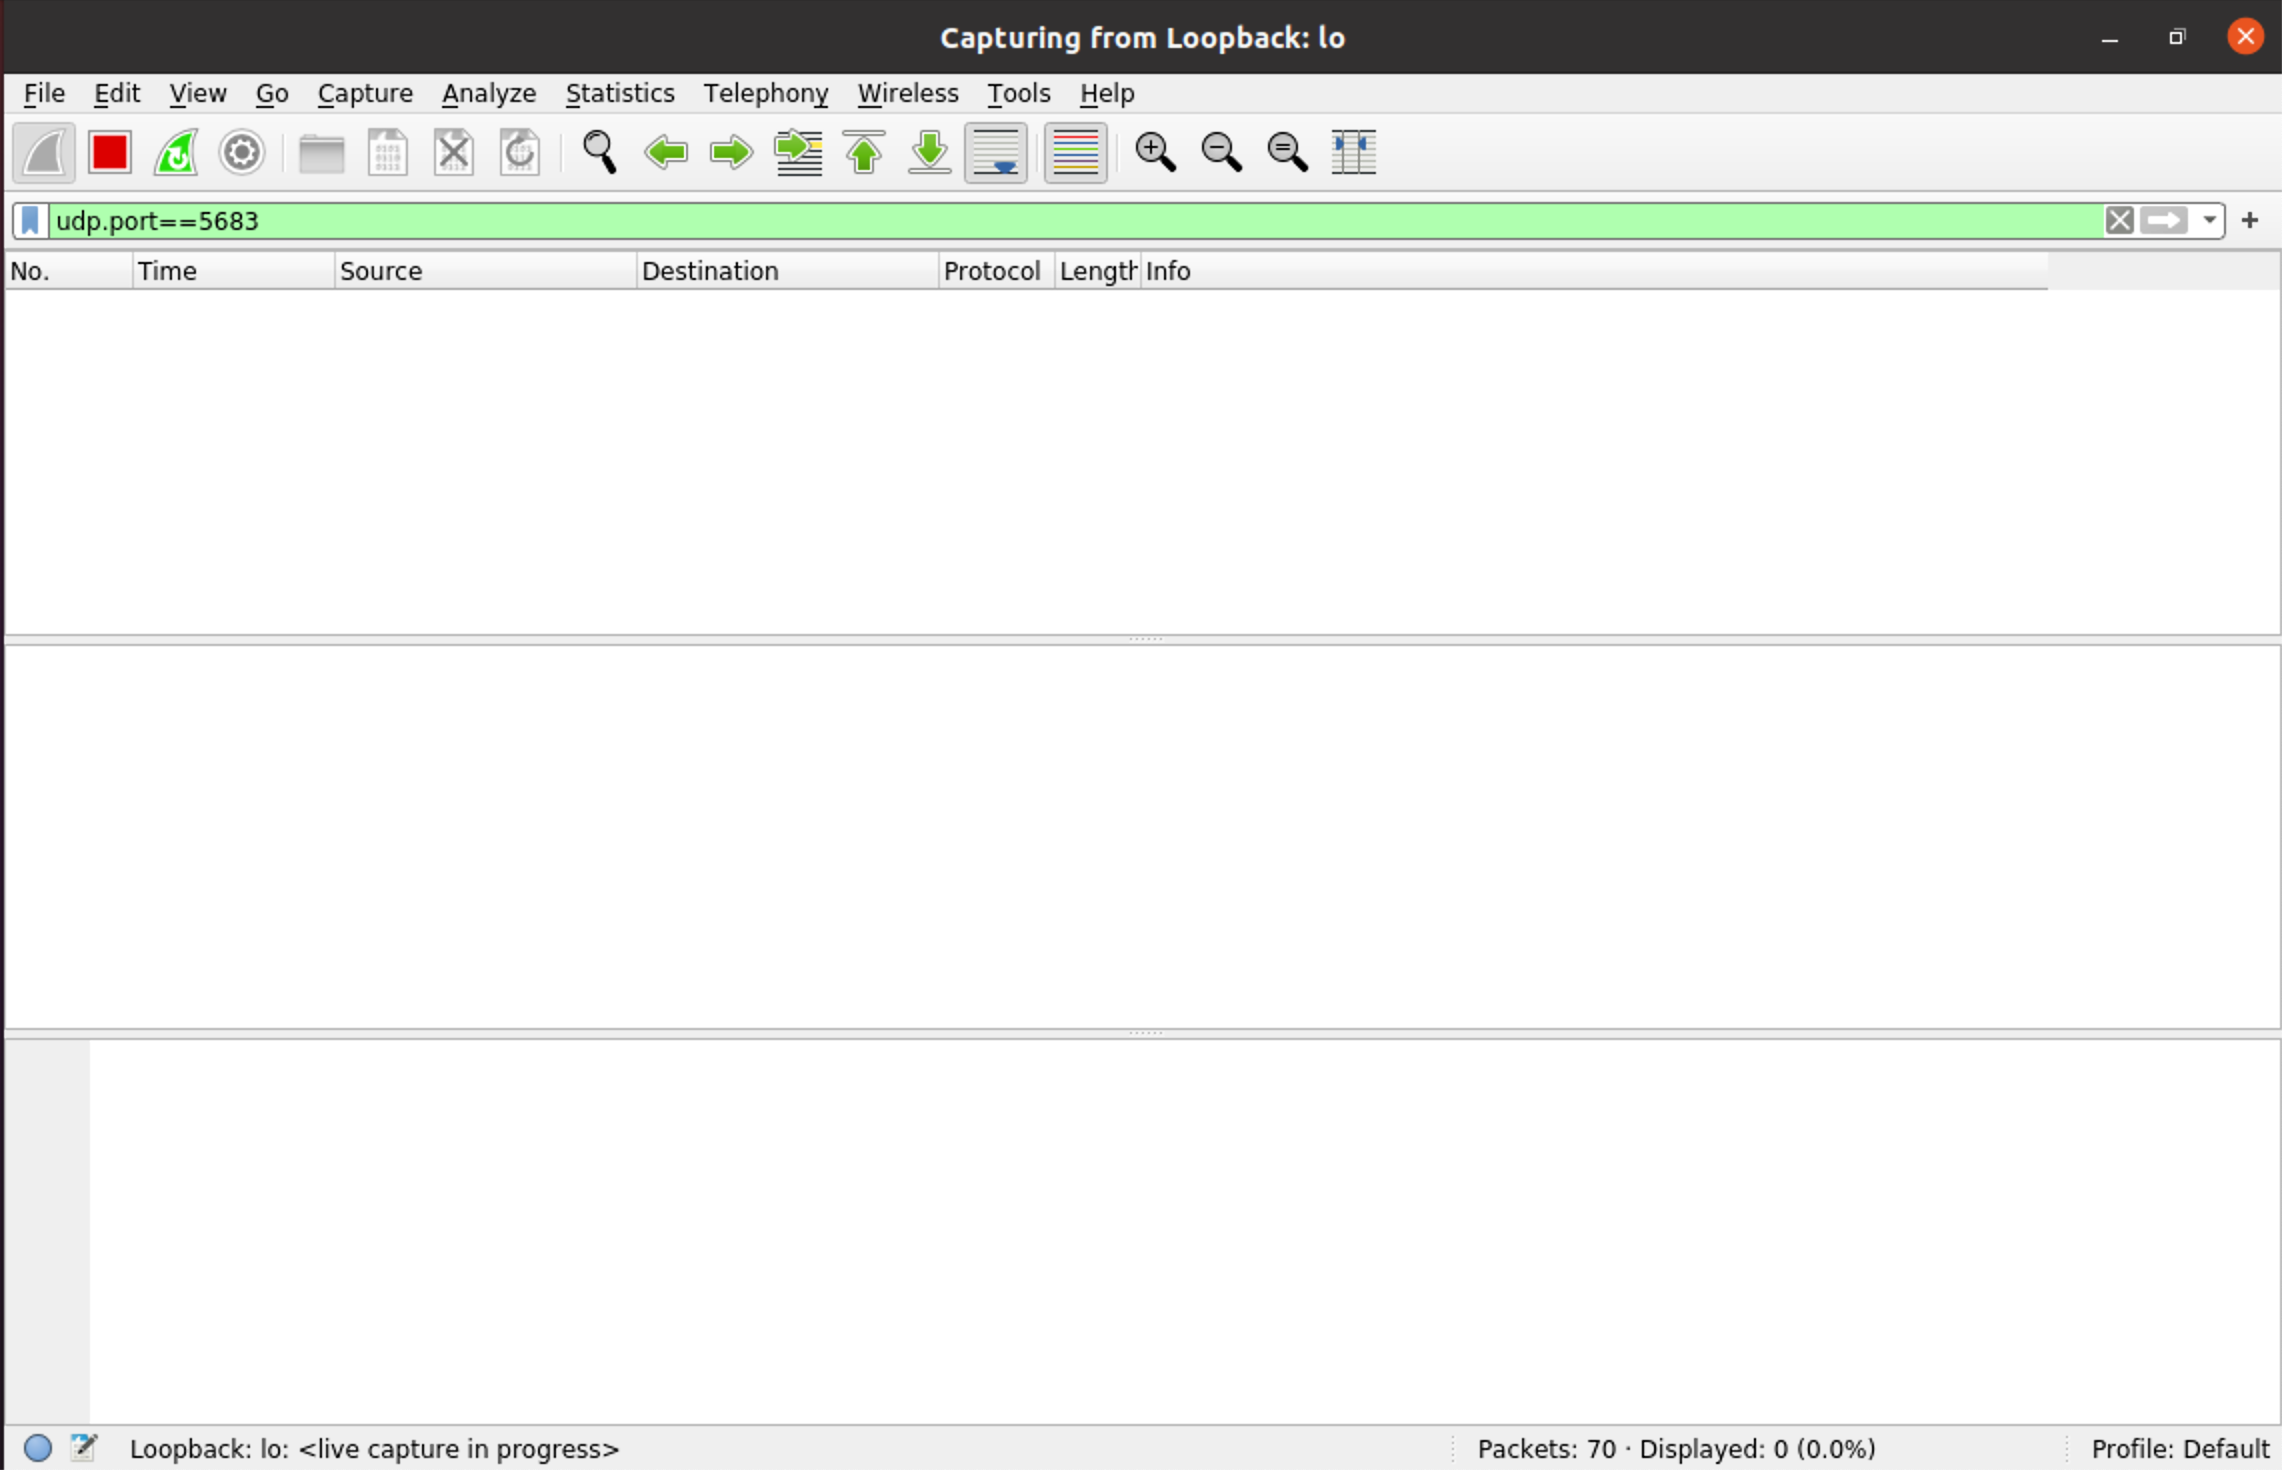
\includegraphics[width=1\columnwidth]{Pictures/lwM2M-wireshark.png}}
\caption{Initialisation de Wireshark pour capturer le trafic CoAP}
\label{fig-lwm2m-wireshark}
\end{figure}

Nous allons maintenant lancer le serveur LwM2M, tapez\footnote{Sous Linux, tapez \texttt{apt install -y default-jre} pour installer Java.}~:

\begin{termc}[backgroundcolor=\color{orange!40}, basicstyle=\ttfamily\small, escapechar=@] % server
> java -jar ./leshan-server-demo.jar
2020-10-22 01:34:09,365 INFO LeshanServer - LWM2M server started at
coap://0.0.0.0/0.0.0.0:5683 coaps://0.0.0.0/0.0.0.0:5684
2020-10-22 01:34:09,553 INFO LeshanServerDemo - Web server started at 
http://0.0.0.0:8080/.
\end{termc}

Il nous indique qu'il utilise le port 5683 pour CoAP et que l'on peut superviser le serveur avec un navigateur sur le port 8080.

         \vspace{1em}

Lancez le navigateur sur l'URI \texttt{http://127.0.0.1:8080}, la page indiqué figure~\vref{fig-lwm2m-server1} apparaît.

\begin{figure}[tbp]
\centerline{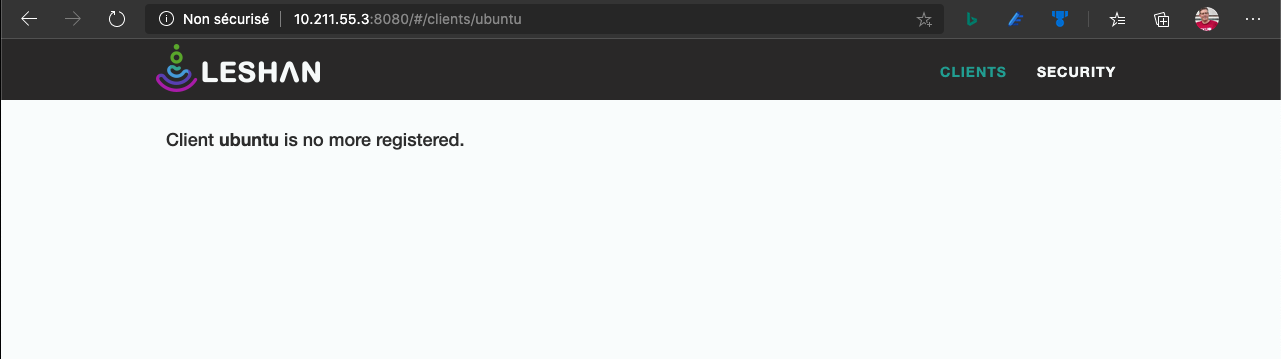
\includegraphics[width=1\columnwidth]{Pictures/lwm2m-server1.png}}
\caption{Page d'accueil du serveur LwM2M}
\label{fig-lwm2m-server1}
\end{figure}

Vous pouvez remarquer que l'ouverture du serveur LwM2M n'a provoqué aucun trafic CoAP sur l'analyseur réseau.

         \vspace{1em}

Lancez maintenant dans une autre fenêtre, le client LwM2M:

\begin{termc}[backgroundcolor=\color{purple!30}, basicstyle=\ttfamily\small, escapechar=@] % client
> java -jar ./leshan-client-demo.jar
2020-10-22 01:49:51,063 INFO LeshanClientDemo - Commands available :

  - create <objectId> : to enable a new object.
  - delete <objectId> : to disable a new object.
  - update : to trigger a registration update.
  - w : to move to North.
  - a : to move to East.
  - s : to move to South.
  - d : to move to West.

2020-10-22 01:49:51,064 INFO LeshanClient - Starting Leshan client ...
2020-10-22 01:49:51,158 INFO CaliforniumEndpointsManager - New 
endpoint created for server coap://localhost:5683 at 
coap://0.0.0.0:48274
2020-10-22 01:49:51,159 INFO LeshanClient - Leshan client
[endpoint:ubuntu] started.
2020-10-22 01:49:51,160 INFO DefaultRegistrationEngine - Trying to 
register to coap://localhost:5683 ...
2020-10-22 01:49:51,252 INFO DefaultRegistrationEngine - Registered 
with location '/rd/BOr5Pg7yW8'.
2020-10-22 01:49:51,252 INFO DefaultRegistrationEngine - Next 
registration update to coap://localhost:5683 in 53s...
\end{termc}

\section{Enregistrement d'un Objet}

Comme nous utilisons une adresse \textit{loopback}, il est un peu plus difficile de repérer dans la trafic Wireshark récupéré (cf. figure~\vref{fig-lwm2m-bootstrap}) qui est le client et qui est le serveur. Mais comme Le serveur attend sur le port 5683, en regarda,t de plus près un paquet, on peut déterminé s'il a été émis par le client ou le serveur.

\begin{figure}[tbp]
\centerline{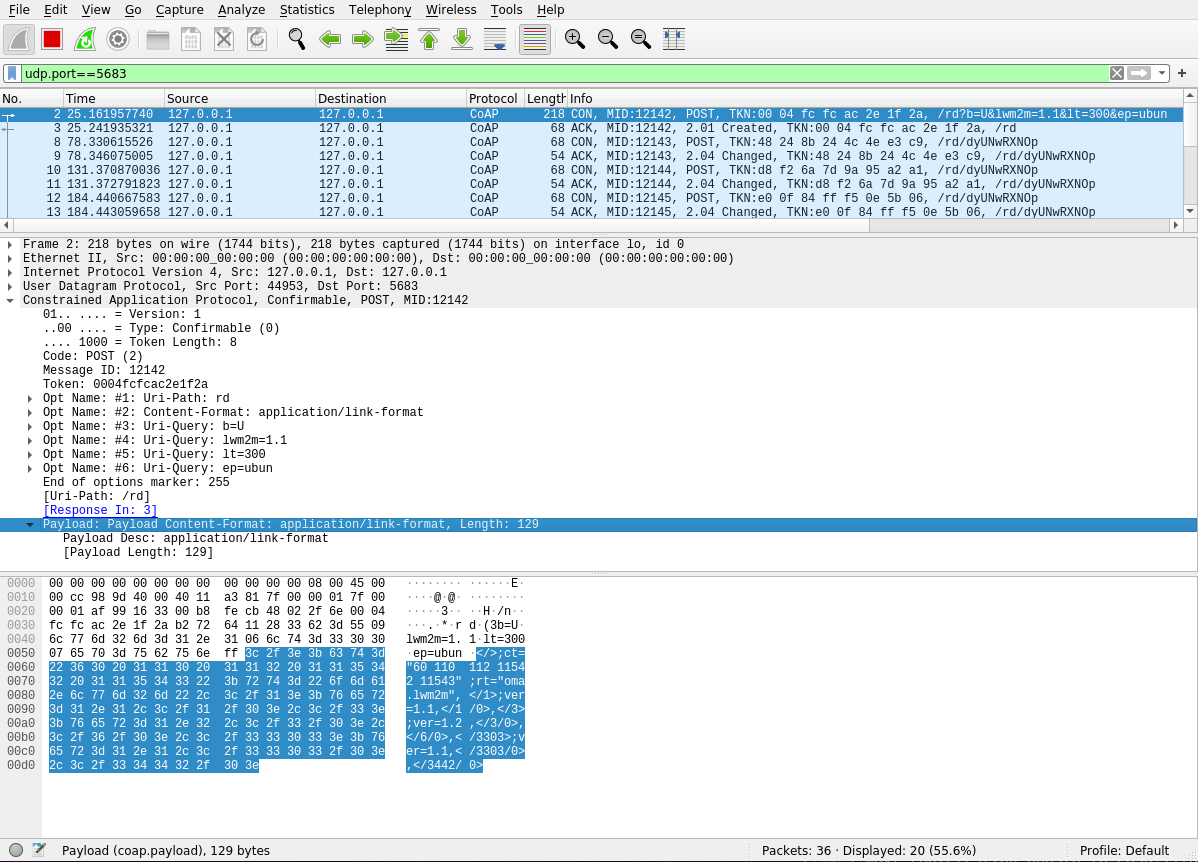
\includegraphics[width=.9\columnwidth]{Pictures/lwm2m-bootstrap.png}}
\caption{Premières captures LwM2M}
\label{fig-lwm2m-bootstrap}
\end{figure}

\subsection{Analyse de l'en-tête CoAP}
On peut voir sur la trace, que le client contacte le serveur pour lui indiquer ses propriétés.

\Question{Méthode}
{Quelle est la nature de la requête émise par le client~:
\begin{itemize}[label=$\circ$]
   \item \Wrong{GET}
   \item \Correct{POST}
   \item \Wrong{PUT}
   \item \Wrong{DELETE}
\end{itemize}}
{
Le client LwM2M agit comme un client REST et envoie cette requête POST~:\\
\noindent\texttt{
Constrained Application Protocol, Confirmable, POST, MID:12142\\
    01.. .... = Version: 1\\
    ..00 .... = Type: Confirmable (0)\\
    .... 1000 = Token Length: 8\\
    Code: POST (2)\\
    Message ID: 12142\\
}
}

\Question{URI}
{Quelle est le chemin de l'URI~:
\begin{itemize}[label=$\circ$]
   \item \Wrong{vide}
   \item \Correct{/rd}
   \item \Wrong{/lwm2m}
\end{itemize}}
{
Le chemin d'URI est composé s'un seul élément~:\\
\noindent\texttt{
    Opt Name: #1: \Index{Uri-Path}: rd\\
}

}

\Question{Content}
{Quelle est le format du contenu (content-format)~:
\begin{itemize}[label=$\circ$]
   \item \Wrong{text}
   \item \Wrong{XML}
   \item \Wrong{JSON}
   \item \Correct{link-format}
   \item \Wrong{CBOR}
\end{itemize}}
{
Après le chemin d'URI on trouve l'option Content-Format qui contient la valeur 40 soit \Index{link-format}~:\\
\noindent\texttt{
    Opt Name: #2: \Index{Content-Format}: application/link-format
}
}

\Question{Période}
{A quelle periode voyez vous d'afficher des messages CoAP ?}
{La figure~\vref{fig-lwm2m-bootstrap} montre plusieurs échanges. Le premier à 25.16 secondes est un POST sur /rd. Le second à 78.33 secondes un POST sur /rd/dyUNwRXNOp. Le troisième à 131.37 secondes est identique et les suivants sont identiques. La période d'envoi est de 53 secondes. }

Pour décoder l'Uri-Query de la requête CoAP il faut d'aider du document \href{http://www.openmobilealliance.org/release/LightweightM2M/V1_1_1-20190617-A/OMA-TS-LightweightM2M_Core-V1_1_1-20190617-A.pdf}{LwM2M Core Specification}\footnote{\url{http://www.openmobilealliance.org/release/LightweightM2M/V1_1_1-20190617-A/OMA-TS-LightweightM2M_Core-V1_1_1-20190617-A.pdf}} et de son tableau 6.2.1 page 40. 


\Question{b=U}{
Que signifie b=U ?
\begin{itemize}[label=$\circ$]
   \item \Wrong{Les données seront émises avec les unités (Units)}
   \item \Wrong{Le référenciel des unités est la représentation Universelle}
   \item \Correct{Le protocole sous-jacent est en mode datagramme (UDP)}
   \item \Wrong{ Le client n'est pas référencé (Unreferenced)}
\end{itemize}
}
{
Ce paramètre désigne le \texitit{binding}, U indique que CoAP sera transporté sur UDP. Le standard propose également d'autres modes, comme~:
\begin{itemize}
    \item T : TCP. CoAP prévoit également un mode de fonctionnement sur \Index{TCP} (\rfc{8323}). Le mode permet par exemple de traverser des réseaux qui restreignent l'usage d'~\Index{UDP} pour de soit disant raisons de sécurité;
    \item S : SMS. LwM2M est défini par l'\acl{OMA}, il est logique d'inclure ce moyen de communication pour gérer un équipement connecté au réseau cellulaire~;
    \item N : \Index{NON-IP}. Dans ce mode, les messages CoAP sont directement envoyés sur le niveau 2. Il est également connu sous le terme de \ac{NIDD} dans les réseaux 4G.
    \item Nous nous basons sur la version 1.1 du standard, la révision 1.2 de LwM2M intègre également de LoRaWAN, MQTT (M), HTTP (H),...
\end{itemize}

~

}


\Question{lwm2m=1.1}{
Que signifie lwm2m=1.1 ? Il s'agit...
\begin{itemize}[label=$\circ$]
   \item \Correct{de la version lwm2m du client}
   \item \Wrong{de la taille mémoire de l'implémentation (1.1 ko)}
   \item \Wrong{de la version lwm2m du serveur}
\end{itemize}
}
{Il s'agit de la version du client. }

\Question{lt=300}{
Que signifie lt=300 ?
\begin{itemize}[label=$\circ$]
   \item \Wrong{C'est le nombre maximal d'objets (less than 300)}
   \item \Wrong{C'est la taille maximale d'un échange (300 octets)}
   \item \Correct{C'est la durée de vie de l'enregistrement d'un objet (lifetime)}
\end{itemize}
}
{C'est la durée de vie d'une valeur, si elle n'est pas rafraîchie avant ce délais par le client, elle disparaîtra du serveur. }

\subsection{Analyse du contenu du POST}

Revenons au contenu du message de la requête POST émise initialement par le client. Que veut dire \Index{link-format}~? Nous n'avons pas encore vu ce format. Heureusement, l'\ac{IANA} est notre ami et en allant chercher à quoi correspond cette valeur, sur cette page \footnote{\url{https://www.iana.org/assignments/core-parameters/core-parameters.xhtml\#content-formats}}, on trouve que le \rfc{6690} définit ce contenu.

Il utilise un format particulier qui est utilisé initialement par le Web pour définir des relations entre pages initialement définit dans le \rfc{5988}. Il est important de remarquer, et après la lecture devient plus claire, que les URI sont notées entre \texttt{<>}. Ensuite, on trouve des attributs liés à cet URI séparés par des points-virgules. Les virgules séparent les définitions.

En suivant ces règles de notation, les données émises par le client peuvent être formatés de la manière suivante :

\begin{termc}[backgroundcolor=\color{purple!30}, basicstyle=\ttfamily\small, escapechar=@] % client
</>;ct="60 110 112 11542 11543";rt="oma.lwm2m",
</1>;ver=1.1,
</1/0>,
</3>;ver=1.2,
</3/0>,
</6/0>,
</3303>;ver=1.1,
</3303/0>,
</3442/0>
\end{termc}

Le client utilise ce format pour décrire les 9 ressources qu'il possède et qui sont identifiées par ces 9 chemins d'URI. Le nommage des ressources peut paraître étrange ; nous verrons par la suite à quoi il correspond~:

\begin{itemize}
    \item La première ligne concerne la racine \texttt{</>} pour laquelle deux attributs sont associés, il seront donc applicable à l'ensemble des éléments. 
    \begin{itemize}
        \item  Le premier \texttt{\Index{ct}}\footnote{Voir \rfc{7252} chapitre 7.2.} définit les formats des représentations possible des objets. La partie entre guillemets fait références aux valeurs de Content-format de CoAP listé tableau~\vref{tab-CoAP-MIME}. On y retrouve respectivement les types CBOR, SenML et pour les deux derniers un format orienté TLV propre à LwM2M.
        \item Le second \texttt{\Index{rt}}\footnote{Voir \rfc{6690} chapitre 3.1.} indique le type de ressource (\textit{resource-type}), c'est-à-dire indique comment elles seront représentées. Ici, cela indique que les ressources suivront les spécifications \ac{LwM2M} de l'\ac{OMA}.
    \end{itemize}
    \item Les lignes suivantes décrivent, toujours de manière hiérarchique, les chemins d'URI et les attributs associés. L'attribut \texttt{\Index{ver}} indique la version du standard utilisée pour définir la ressource.
 
\end{itemize}


\Question{rt}{
À quoi sert l'attribut rt ?
\begin{itemize}[label=$\circ$]
   \item \Correct{à donner la sémantique (i.e. comment interpréter) de la ressource.}
   \item \Wrong{à indiquer la taille de la ressource en faisant référence à lwm2m.}
   \item \Wrong{ à indiquer la version de lwm2m utilisée.}
   \item \Wrong{à aider à déboguer les échanges.}
\end{itemize}
 }{
 Quand le serveur reçoit le POST du client, il est capable d'associer une représentation au chemin d'URI décrit. Le client et le serveur doivent avoir cette connaissance à priori.
 }

\subsection{Définition des ressources}

LwM2M représente les ressources d'une manière assez originale pour être à la fois compact, universel (ce qui est quelquefois oxymorique) et flexible. Pour ce faire, tout est désigné par des chiffres.  Le chapitre 7 page 63 du document. principal\footnote{\url{http://www.openmobilealliance.org/release/LightweightM2M/V1_1_1-20190617-A/OMA-TS-LightweightM2M_Core-V1_1_1-20190617-A.pdf}} contient le schéma figure~\vref{fig-lwm2m-objects}  illustrant cette hiérarchie~:  

\begin{figure}[tbp]
\centerline{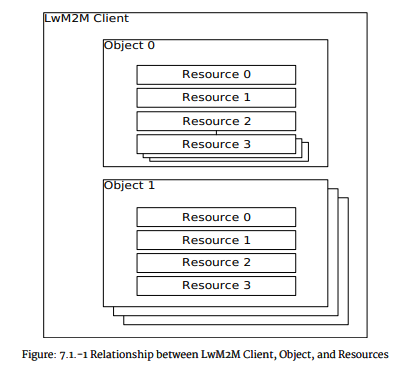
\includegraphics[width=.6\columnwidth]{Pictures/lwm2m-objects.png}}
\caption{Hierarchie de nommage}
\label{fig-lwm2m-objects}
\end{figure}

\begin{itemize}
\item Un Objet physique (ie notre client) contient une liste d'objets numériques\footnote{LwM2M appelle cette information \textit{object} ce qui rend en français la définition ambiguë puisque Objet est aussi la traduction de \textit{thing}} identifié par un numéro. Ce numéro est attribué par l'OMA. Par exemple, un capteur de température aura la valeur \textit{\textttt{3303}}. Une liste des valeurs déjà attribuées peut être trouvée à cette \href{http://www.openmobilealliance.org/wp/OMNA/LwM2M/LwM2MRegistry.html#resources}{adresse}\footnote{\url{http://www.openmobilealliance.org/wp/OMNA/LwM2M/LwM2MRegistry.html#resources}}. 
\item Un client peut évidemment posséder plusieurs instance d'un objet numérique, par exemple, une station météo pourrait avoir un capteurs de température intérieur et extérieur. Le deuxième chiffre du chemin de l'URI indique cette instance. S'il n'y en a qu'un, il prend la valeur \textit{\textttt{0}}.
\item Finalement, l'objet peut être complexe et contenir plusieurs informations appelée ressouces. En cliquant sur le chiffre \textit{\textttt{3303}} dans la page web précédente, on obtient la description de l'objet. On peut voir que :
\begin{itemize}
\item \textit{\textttt{5700}} représente la valeur mesurée par le capteur
\item \textit{\textttt{5601}} la valeur minimale
\item \textit{\textttt{5602}} la valeur maximale
\item \textit{\textttt{5701}} indique les unités 
\item \textit{\textttt{5605}} permet de remettre à zéro le calcul des minima et maxima
\end{itemize}
Ces valeurs peuvent se retrouver dans plusieurs objets numériques.
\item la version 1.2 du standard introduit également la possibilité d'avoir plusieurs instances d'une ressource.
\end{itemize}

\subsubsection{Valeurs associées aux objets numériques}
Les objets numériques peuvent être définit par LwM2M, ils concernent ceux dédié à la gestion du protocole. Par exemple, l'objet numérique~:

\begin{itemize}
    \item  \textit{\textttt{0}} définit l'environnement de sécurité du client. Il contient l'adresse du serveur, les clés de chiffrement,\ldots
    \item \textit{\textttt{1}} définit les paramètres pour la communication avec le serveur, comme par exemple la durée de vie de l'information en seconde,\ldots
    \item \textit{\textttt{3}} décrit les caractéristiques de l'équipement comme sa version logicielle,\ldots
    \item \ldots
\end{itemize}

         \vspace{1em}


Les valeurs comprises entre 2~048 et 10~240 sont définies par des organismes de standardisation partenaire de l'\ac{OMA},  comme par exemple~:
\begin{itemize}
    \item l'\acro{IPSO} Alliance qui va définir des objets numériques types, comme un capteur de température ayant pour référence \textit{\textttt{3303}},
    \item la \acro{GSMA} qui définit les objets pour la gestion des téléphones cellulaire,
    \item \ldots
\end{itemize}

Les valeurs supérieures sont réservées aux industriels qui peuvent enregistrer leurs propres spécifications.

\subsubsection{Valeurs associées aux ressources}

La figure~\vref{fig-lwm2m-3303}, copiée du site Web de l'\ac{OMA}, donne un exemple de définition d'un objet numérique. A l'objet 3303 sont associés un certain nombre de ressources, générique que l'on peut aussi trouver dans d'autres objets numérique. Ainsi~:

\begin{figure}[tbp]
\centerline{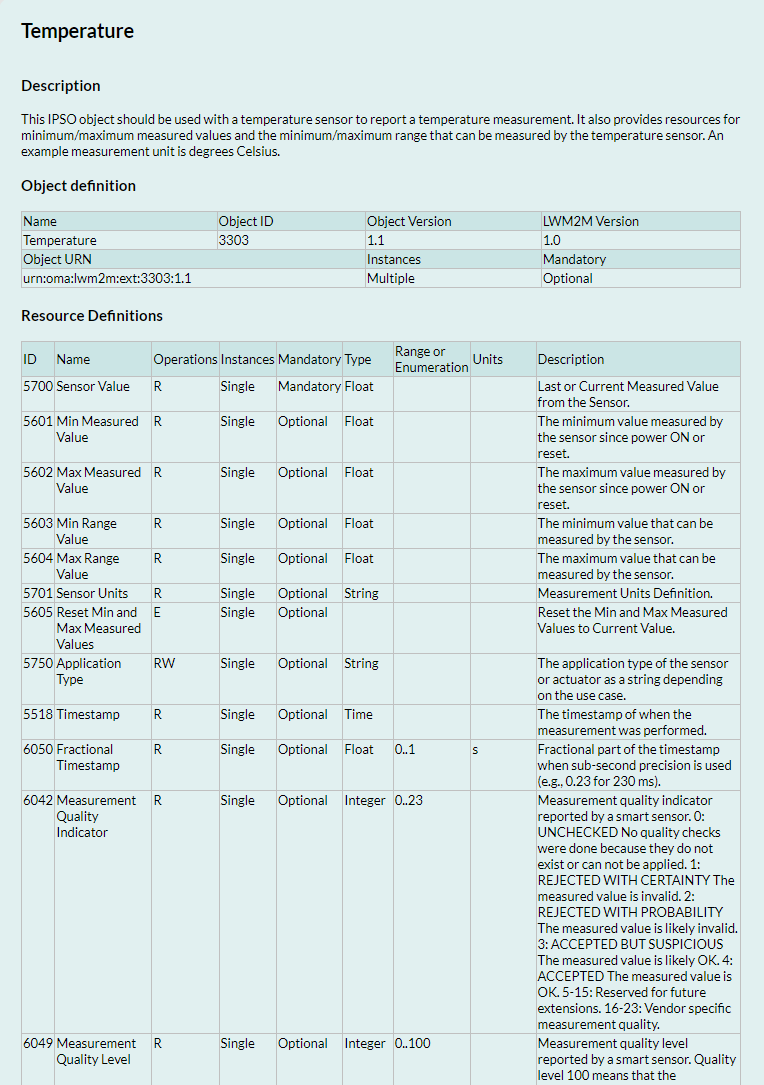
\includegraphics[width=1\columnwidth]{Pictures/lwm2m-3303.png}}
\caption{Définition de l'objet numérique 3303 pour la température}
\label{fig-lwm2m-3303}
\end{figure}

\begin{itemize}
    \item \textit{\textttt{5700}} fait référence à la valeur mesurée représenté comme un nombre flottant. Ce nombre ne peut que être lu (\texttt{R})
    \item \textit{\textttt{5700}} est une chaîne de caractère qui précise l'unité de mesure.
    \item \textit{\textttt{5601}} et \textit{\textttt{5602}} conservent les valeurs minimales et maximales. Elle peuvent être remise à zéro via la ressource \textit{\textttt{5605}} qui conduit à une exécution d'un programme (\texttt{E}).
    \item les \textit{\textttt{5603}} et \textit{\textttt{5604}} valeurs correspondent à la plage d'utilisation du capteur et ne peuvent pas être modifiées.
\end{itemize}


         \vspace{1em}
         
Ainsi \textit{\texttt{3303/3/5601}} représente la valeur minimale (\textit{\textttt{5601}}) du quatrième capteur (\textit{\textttt{3}} car on commence à 0) de l'objet numérique température (\textit{\textttt{3303}}).

Par rapport à \Index{Modbus}, où l'on devait télécharger la documentation de l'Objet (cf tableau~\vref{tab-meter-IR}), LwM2M offre une manière standard de décrire l'information produite ou consommée par un Objet. De plus, la définition de l'objet numérique, en plus d'être visualisable sous forme de tableau sur le site web, existe aussi en \Index{XML} pour être traitée informatiquement et permettre l'interopérabilité.

\begin{termc}[backgroundcolor=\color{blue!10}, basicstyle=\ttfamily\tiny, escapechar=@, language=xml] % client
<?xml version="1.0" encoding="UTF-8"?>

<!-- BSD-3 Clause License ... -->

<LWM2M  xmlns:xsi="http://www.w3.org/2001/XMLSchema-instance" xsi:noNamespaceSchemaLocation=
"http://openmobilealliance.org/tech/profiles/LWM2M.xsd">
	<Object ObjectType="MODefinition">
		<Name>Temperature</Name>
		<Description1>
		    This IPSO object should be used with a temperature sensor to report a temperature
		    measurement.  It also provides resources for minimum/maximum measured values and the
		    minimum/maximum range that can be measured 
		    by the temperature sensor. An example measurement unit is degrees Celsius.
		</Description1>
		<ObjectID>3303</ObjectID>
		<ObjectURN>urn:oma:lwm2m:ext:3303:1.1</ObjectURN>
		<LWM2MVersion>1.0</LWM2MVersion>
		<ObjectVersion>1.1</ObjectVersion>
		<MultipleInstances>Multiple</MultipleInstances>
		<Mandatory>Optional</Mandatory>
		<Resources>
			<Item ID="5700">
				<Name>Sensor Value</Name>
				<Operations>R</Operations>
				<MultipleInstances>Single</MultipleInstances>
				<Mandatory>Mandatory</Mandatory>
				<Type>Float</Type>
				<RangeEnumeration></RangeEnumeration>
				<Units></Units>
				<Description>Last or Current Measured Value from the Sensor.</Description>
			</Item>
			<Item ID="5601">
				<Name>Min Measured Value</Name>
				<Operations>R</Operations>
				<MultipleInstances>Single</MultipleInstances>
				<Mandatory>Optional</Mandatory>
				<Type>Float</Type>
				<RangeEnumeration></RangeEnumeration>
				<Units></Units>
				<Description>
				  The minimum value measured by the sensor since power ON or reset.
				  </Description>
			</Item>
			...
\end{termc}

\Question{3301/0/5602}{En vous aidant de la \href{http://www.openmobilealliance.org/wp/OMNA/LwM2M/LwM2MRegistry.html#resources}{page de decription des objets numériques et des ressources}\footnote{\url{http://www.openmobilealliance.org/wp/OMNA/LwM2M/LwM2MRegistry.html#resources}}, que représente l'URI \textit{\texttt{3301/0/5602}}?
\begin{itemize}[label=$\circ$]
   \item \Wrong{la température maximale du premier capteur}
   \item \Wrong{l'humidité minimale du capteur 0}
   \item \Correct{la luminosité maximale du capteur 0}
\end{itemize}
}{
En allant sur la page web, on trouve que \textit{\texttt{3301}} correspond à la mesure de la luminosité {\textit{Illuminance})}. La description de cet objet numérique est identique à celle de l'objet numérique \textit{temperature}~; \textit{\texttt{3301/3/5602}} indique la valeur maximale.
}

\Question{10340/0/2}{
Que représente l'URI \textit{\texttt{10340/0/2}}?
\begin{itemize}[label=$\circ$]
   \item \Wrong{la température en Fahrenheit de l'objet 10340}
   \item \Wrong{la longitude dans des coordonnées GPS }
   \item \Correct{le statut actif ou non d'une caméra }
\end{itemize}
}{
En allant sur la page web, on trouve que \textit{\texttt{10340}} correspond à un objet numérique \textit{Camera} définit par la société \texitit{CloudMinds}. La description de cet objet numérique montre que la ressource \textit{\texttt{2}} correspond au status (\textit{1:Enabled, 0:Disabled}.)
}

\Question{Dimmer}
{Quelle URI permet d'accéder à l'élément contrôlant la variation lumineuse (\textit{Dimmer}) d'un éclairage (\textit{Light Control}) ? Quelle valeur maximale peut prendre cette ressource ? }
{\textit{\texttt{3311/0/5851}} La valeur maximale est de 100.
}

\Question{Hz} {Quel serait le chemin d'URI pour obtenir la fréquence d'un courant électrique sur la deuxième phase ?}
{
\textit{\texttt{3318/1/5700}} 
}

\Question{Qui est qui?}
{Dans le premier échange capturé~:\\
\\
\texttt{
</>;ct="60 110 112 11542 11543";rt="oma.lwm2m",\\
</1>;ver=1.1,\\
</1/0>,\\
</3>;ver=1.2,\\
</3/0>,\\
</6/0>,\\
</3303>;ver=1.1,\\
</3303/0>,\\
</3442/0>\\
}
\ifthenelse{\boolean{Response}}{
\begin{description}
    \item    \tab 1 $\square$ \tab$\square$ Location
    \item    \tab 3 $\square$ \tab $\square$ Device
    \item    \tab 6 $\square$ \tab$\square$ LwM2M v1.1 Test Object
    \item    \tab 3303 $\square$ \tab $\square$ LwM2M Server
    \item    \tab 3442 $\square$ \tab $\square$ Temperature
\end{description}
}{}
}
{
\begin{description}
    \item 1: Device 
    \item 3: LwM2M Server
    \item 6: Location
    \item 3303: Temperature
    \item 3442: LwM2M v1.1 Test Object
\end{description}
}

\section{\textit{Resource Directory}}

Nous allons nous focaliser sur le premier échange que nous avons commencé à analyser en regardant le message émis par le client vers le serveur LwM2M. Comme nous l'avons vu, ce premier message contient la description des ressources présentes sur le client. Les valeurs des identifiants d'objets numérique (Object ID) et de ressources (Resource ID) permettent au serveur de savoir ce que peut faire le client, vu qu'elles sont normalisées. Le client LwM2M envoie ces informations sur un chemin d'URI bien connu \texttt{/rd} (pour \textit{resource description}).

\begin{figure}[tbp]
\centerline{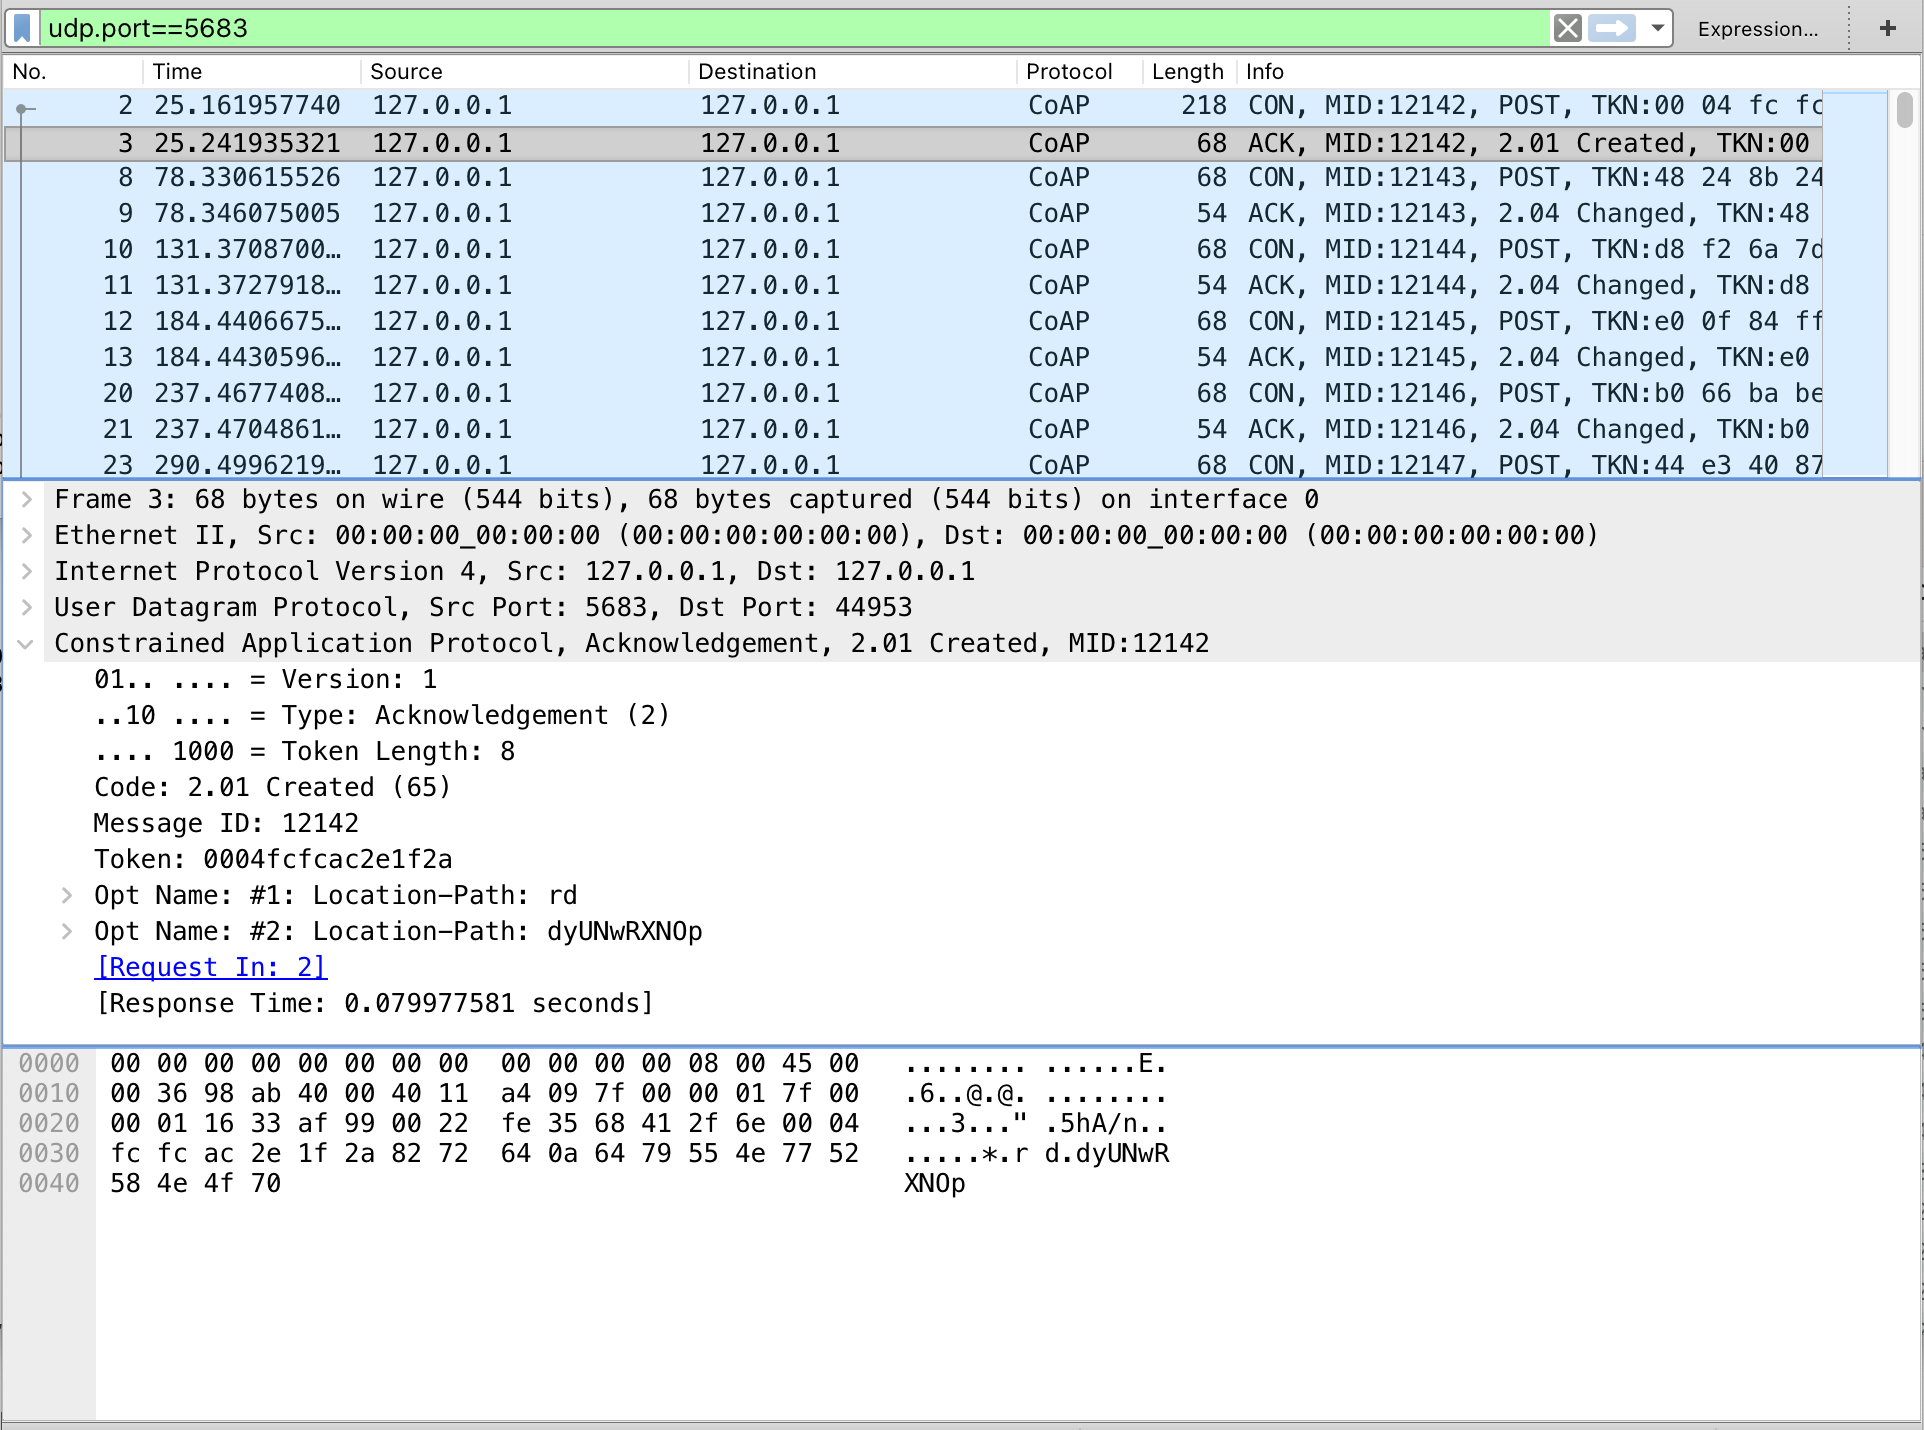
\includegraphics[width=.8\columnwidth]{Pictures/lwm2m-rep.png}}
\caption{Réponse du serveur LwM2M au POST du client}
\label{fig-lwm2m-rep}
\end{figure}

\Question{Réponse du serveur LwM2M}
{
Que répond le serveur (cf. figure~\vref{fig-lwm2m-rep})?
\begin{itemize}[label=$\circ$]
   \item \Wrong{Il acquitte juste le message.}
   \item \Wrong{Rien.}
   \item \Correct{Il renvoie une URI qui servira par la suite à identifier l'objet.}
   \item \Wrong{Il retourne les données de chiffrement des messages.}
\end{itemize}
}{
La réponse contient l'option \textit{\Index{Location-Path}} ce qui permet de préciser où la ressource fournie par la client a été référencée sur le serveur. Comme pour \textit{\Index{URI-Path}}, il s'agit d'une option qui peut se répéter. Dans l'exemple,  figure~\vref{fig-lwm2m-rep}, l'URI fournie est donc \texttt{/rd/dyUNwRXNOp}.

Cette URI servira par la suite d'identifiant interne pour le client.
}
 
 \Question{Wait and See}
 {
 Si on laisse la plate-forme fonctionner sans intervenir, que voit-on sur l'analyseur réseau ?
 
 \begin{itemize}[label=$\circ$]
   \item \Wrong{ Rien.}
   \item \Wrong{Le capteur envoie des informations indiquant un changement de valeur mesurée.}
   \item \Wrong{Le client envoie les valeurs mesurées même s'il elles n'ont pas changé.}
   \item \Correct{Le client envoie un message vide vers le serveur pour indiquer qu'il est toujours présent.}
   \item \Wrong{ Le serveur envoie un message vide vers ses clients pour savoir s'ils sont toujours présents.}
\end{itemize}
}{
Toutes les 53 secondes, le client envoie un POST vers la ressource créée à l'enregistrement. Ce POST est vide. Il sert à indiquer au serveur que le serveur est toujours présent. Le serveur acquitte ce message indiquant au client qu'il est aussi accessible.
}
  
\section{interrogation du client LwM2M}

Il est temps de revenir à l'interface de la plate-forme en ouvrant la page \texttt{http://127.0.0.1:8080} depuis le navigateur. Assurez vous que Wireshark capture toujours le trafic sur l'interface \textit{loopback}.  L'objet que nous avons inscrit apparaît. Cliquez dessus. Vous devez avoir quelque chose comme ce qui est représenté figure~\vref{fig-lwm2m-obs}.


\begin{figure}[tbp]
\centerline{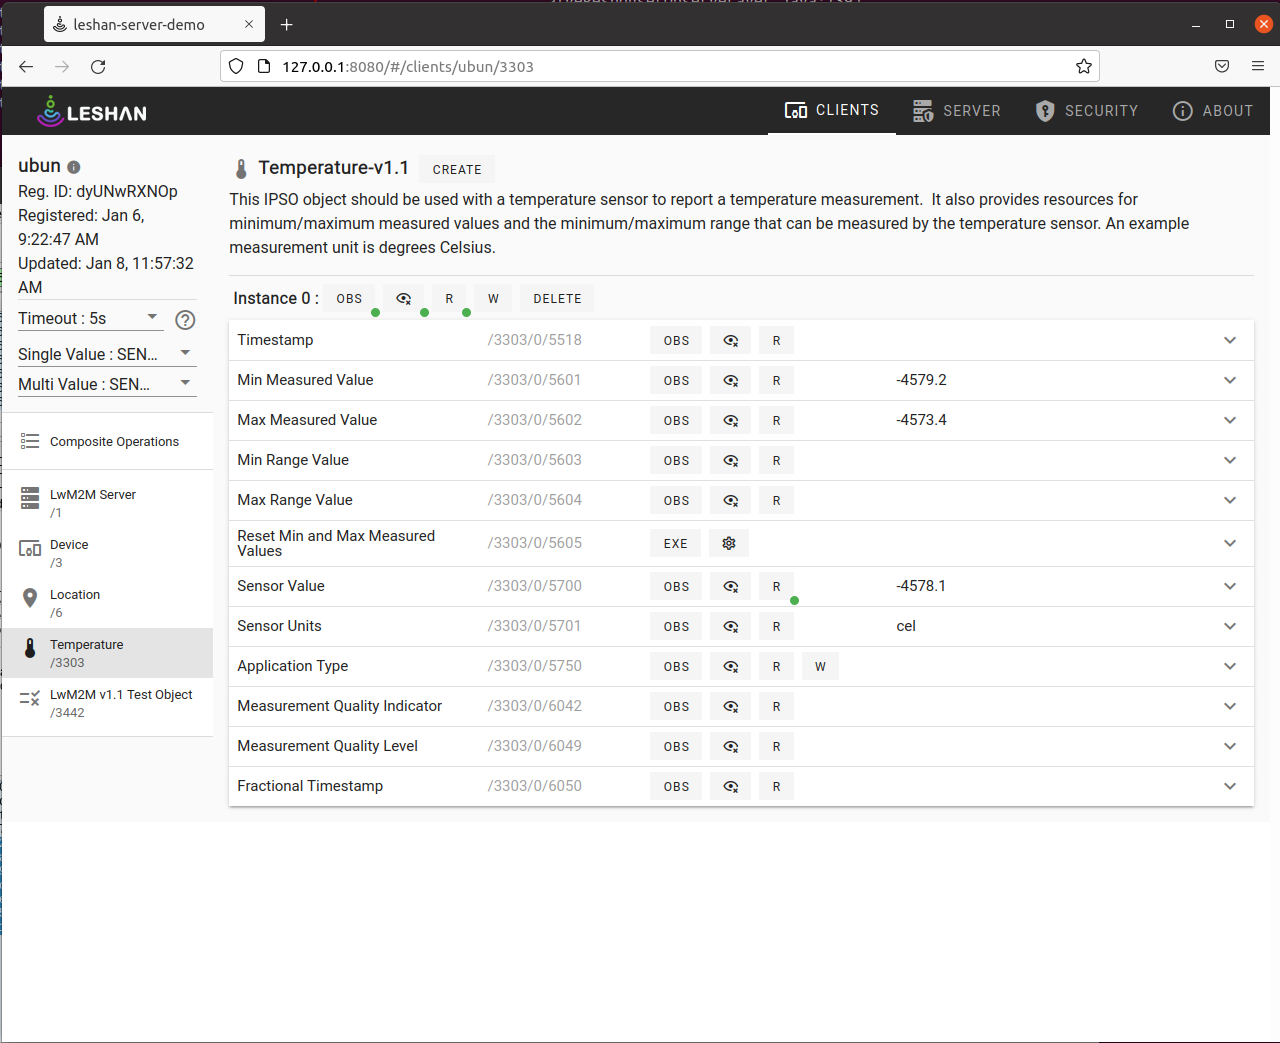
\includegraphics[width=1\columnwidth]{Pictures/lwm2m-obsever.png}}
\caption{Visualisation du serveur LwM2M}
\label{fig-lwm2m-obs}
\end{figure}

         \vspace{1em}

Dans le menu de gauche, on retrouve les objets numérique LwM2M décrit lors du premier POST de l'Objet.

         \vspace{1em}

En cliquant sur \textit{Temperature}, les ressource LwM2M sont affichées. Les petits logos permettent d'effectuer des actions~:
\begin{itemize}
    \item \texttt{\textit{R}} pour lire une ressource, \texttt{\textit{W}} pour l'écrire et \texttt{\textit{EXE}} pour exécuter un code (l'engrenage permet de définir les paramètres)~;
    \item \texttt{\textit{OBS}} permet de lancer un \Index{Observe} sur une ressource, L'oeil avec la croix permet d'annuler un Observe.
\end{itemize}
Ces actions peuvent s'appliquer individuellement à chaque ressource, ou plus globalement à une instance d'un objet numérique.

\subsection{Lecture simple}

Dans le menu du gauche, sélectionnez \texit{SENML\_JSON} dans le menu déroulant \textit{Single Value}. Cela permettra d'utiliser le format \Index{SenML} plutôt que celui spécifié par LwM2M basé sur des \ac{TLV}. 

         \vspace{1em}

Pour l'objet numérique \textit{Temperature} cliquez sur le bouton \texttt{\textit{R}} de \textit{Sensor Value}. La figure~\vref{fig-lwm2m-get-simple} monte cet échange et détaille la réponse.
Le Serveur LwM2M agit comme un client REST et envoie au serveur REST du client LwM2M la requête~:

\begin{figure}[tbp]
\centerline{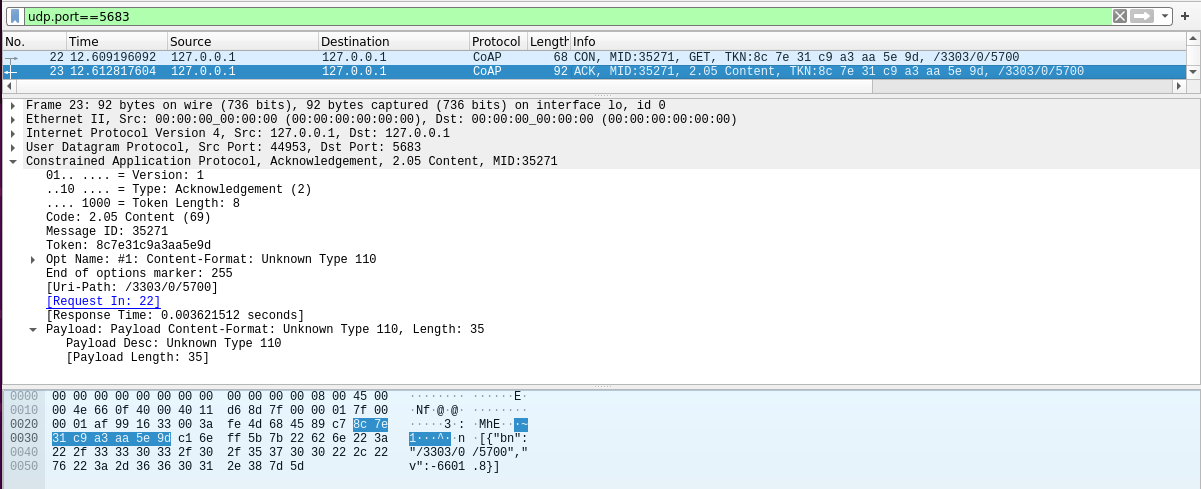
\includegraphics[width=1\columnwidth]{Pictures/lwm2m-get-simple.png}}
\caption{Interrogation d'une ressource}
\label{fig-lwm2m-get-simple}
\end{figure}

\begin{termc}[backgroundcolor=\color{orange!40}, basicstyle=\ttfamily\small, escapechar=@] % server
GET /3303/0/5700 
\end{termc}

\noindent en indiquant le type \texttt{110} dans l'option \Index{Accept} (cf. tableau~\vref{tab-CoAP-MIME}) qui correspond au format \Index{SenML} codé en JSON . 


         \vspace{1em}


La réponse doublement associée par le même \Index{Token} et un message de type \Index{ACK} de format SenML en JSON~:  


\begin{termc}[backgroundcolor=\color{purple!30}, basicstyle=\ttfamily\small, escapechar=@] % client
[{"bn":"/3303/0/5700","v":-6601.8}]
\end{termc}

On y retrouve le nom de base (\texttt{\Index{bn}}) correspondant au nom de la ressource et la valeur (\texttt{\Index{v}})\footnote{Il est évident que le résultat retourné n'a aucun sens physique, le client LwM2M émulant mal l'évolution d'une température sur le long terme.}.

          \vspace{1em}

Cette valeur s'affiche dans la page web du serveur LwM2M, le petit point vert indiquant que l'échange s'est déroulé correctement (cf. figure~\vref{fig-lwm2m-temp-simple}).

\begin{figure}[tbp]
\centerline{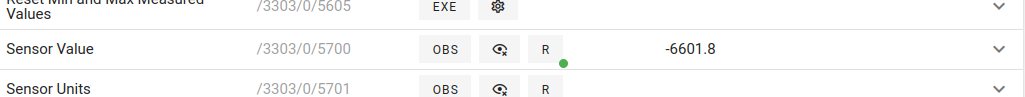
\includegraphics[width=1\columnwidth]{Pictures/lwm2m-temp-simple.png}}
\caption{Relevé de la température}
\label{fig-lwm2m-temp-simple}
\end{figure}

\subsection{Lecture d'une instance}

En  sélectionnant \texit{SENML\_JSON} dans le menu déroulant \textit{Multi Value} et en cliquant sur le bouton \texttt{\textit{R}} à droite de \textit{\textbf{Instance 0}}, différents champs de l'instance se remplissent. 

L'échange protocolaire est similaire à précédent. Le serveur LwM2M a émis la requête suivante, où la valeur de la ressource est omis~:

\begin{termc}[backgroundcolor=\color{orange!40}, basicstyle=\ttfamily\small, escapechar=@] % server
GET /3303/0
\end{termc}

\noindent et la réponse contient~:

\begin{termc}[backgroundcolor=\color{purple!30}, basicstyle=\ttfamily\small, escapechar=@] % client
[{"bn":"/3303/0/","n":"5601","v":-6672.6},
{"n":"5602","v":-4573.4},
{"n":"5700","v":-6671.6},
{"n":"5701","vs":"cel"}]
\end{termc}

On remarque que le nom de base  (\texttt{\Index{bn}})correspond à l'URI de l'instance et que chaque éléments contient un champs nom  (\texttt{\Index{n}}) contient l'identifiant numérique de la ressource\footnote{Le champ  (\texttt{\Index{vs}}) indique que le contenu doit être interprété comme une chaîne de caractères}.

\subsection{Observe}

Il est aussi possible de suivre dans le temps l'état d'une ressource, nous allons le faire pour la ressource \textit{Sensor Value} de l'objet numérique \textit{Temperature}. Cliquez sur le bouton \texttt{\textit{OBS}}.

Le serveur LwM2M émet la requête GET comme précédemment, en ayant inséré la l'option \textit{\Index{Observe}} avec la valeur 0 pour indiquer qu'il souhaite recevoir périodiquement des informations. Les réponses incluent également une option \textit{\Index{Observe}}  dont la valeur est croissante.

Sur Wireshark, vous pourrez vérifier que périodiquement la réponse est envoyée en utilisant un message de type \textit{\Index{CON}firmable} plutôt que \textit{\Index{NON} confirmable} pour vérifier que le client REST sur le serveur LwM2M est toujours actif (cf figure~\vref{fig-lwm2m-obs-con})

\begin{figure}[tbp]
\centerline{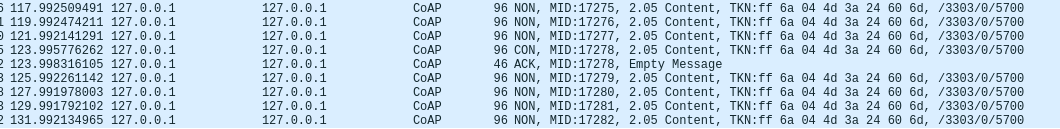
\includegraphics[width=1\columnwidth]{Pictures/lwm2m-observe-con.png}}
\caption{Emission d'un Observe avec un message CONfirmable}
\label{fig-lwm2m-obs-con}
\end{figure}

\Question{Fin d'observe}
{Un click sur l'oeil avec la croix permet au serveur d'annuler l'Observe. Quel message est émis ?}
{Quand le serveur LwM2M reçoit un Observe pour une session qui a été annulée, il répond avec un message de type \textit{ReSeT}, la valeur du champ \textit{Message ID} permet au client LwM2M de savoir quelle session d'Observe annuler.
}

\Question{EXE}
{Quel message est émis, si on clique sur une ressource de type EXE, comme la remise à zéro des valeurs min et max?}
{Cela ne change rien au protocole, un POST sur l'URI de la ressource est émis par le serveur LwM2M.}